%%
%% Implementation
%%

\chapter{Implementation}

Thist chapter \ldots

\section{System Overview}
\begin{figure}[h]
	\begin{center}
		{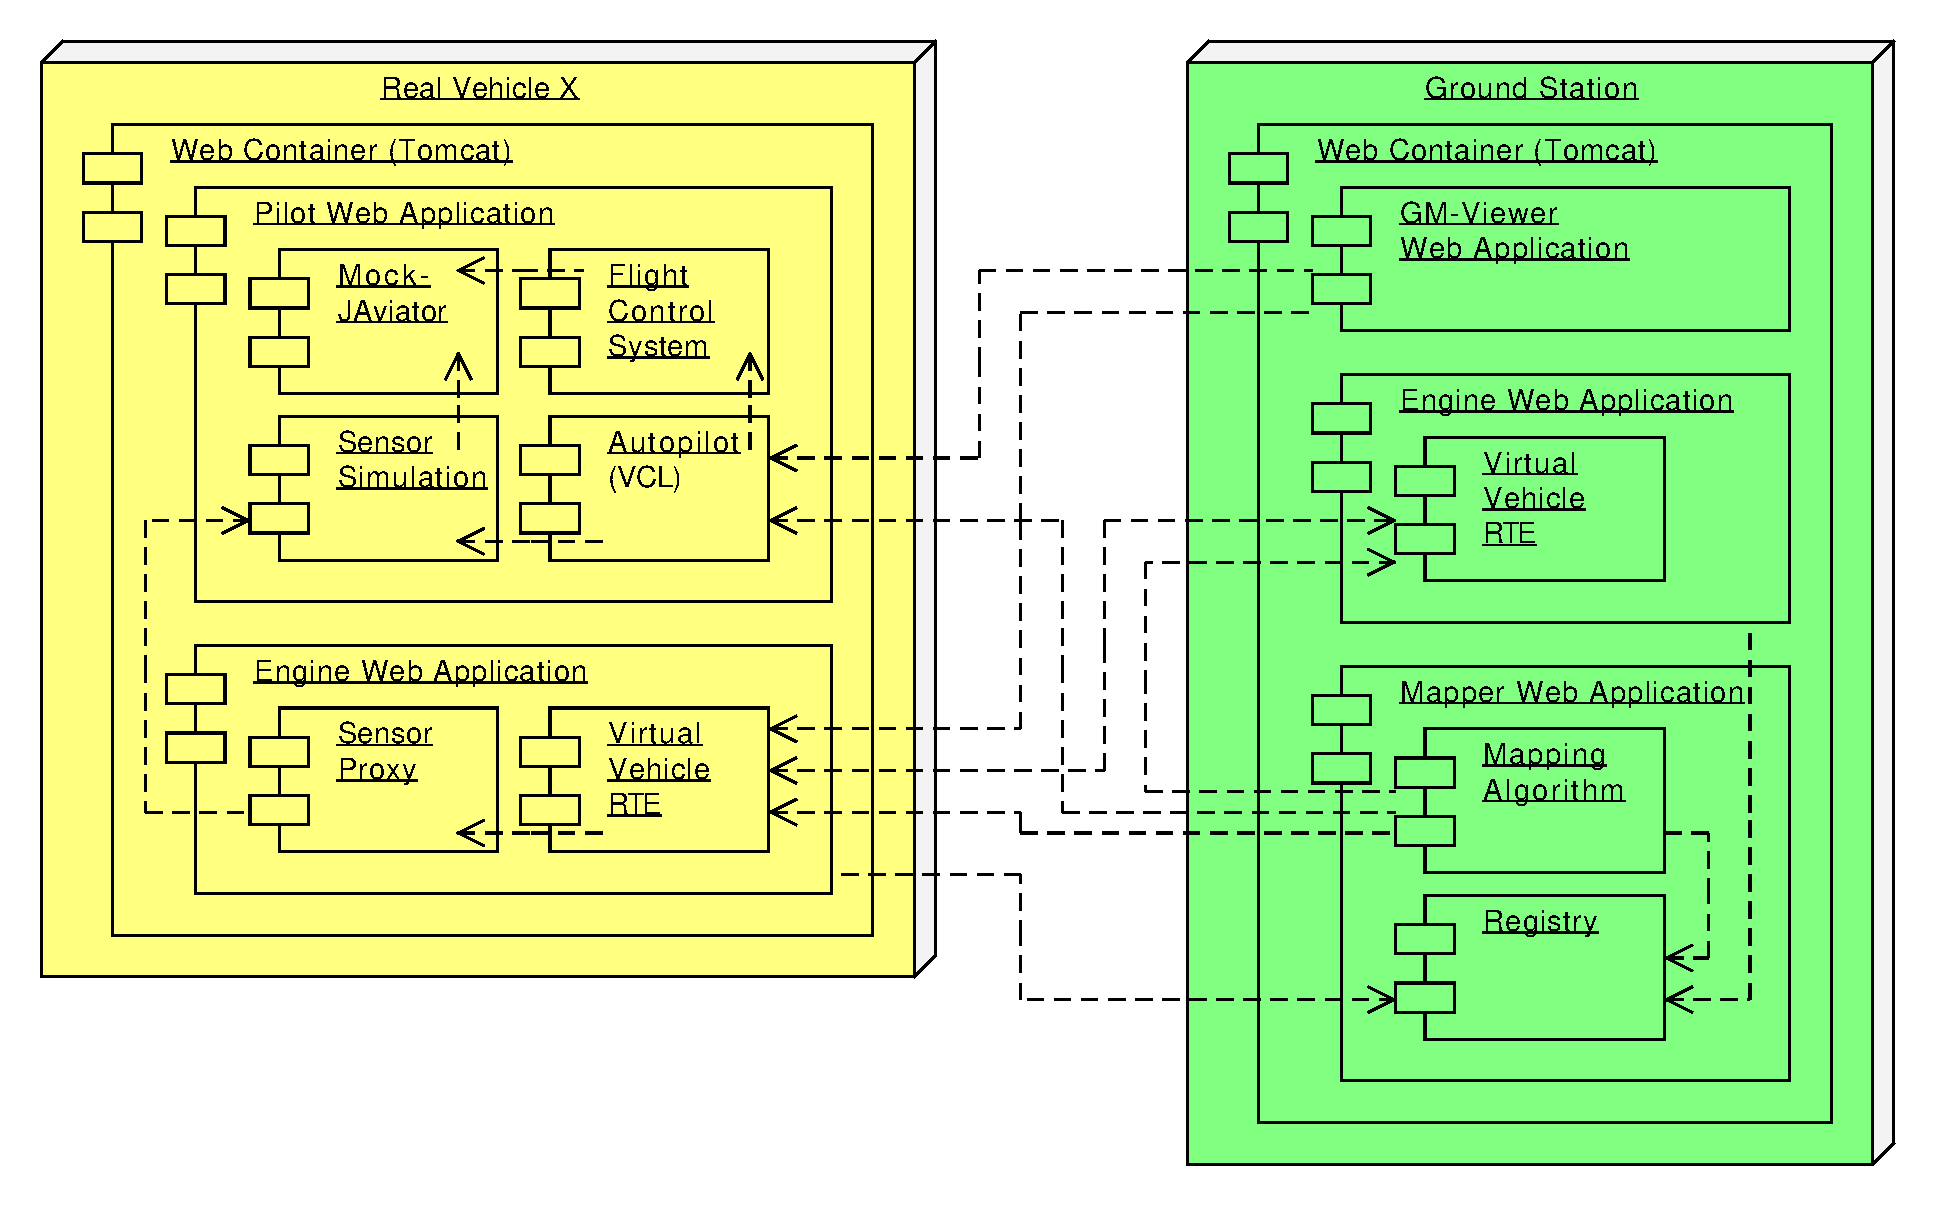
\includegraphics[width=10cm]{SystemOverview.pdf}}
	\end{center}
	\caption{System Overview.\label{fig:SystemOverview}}
\end{figure}


\section{Sensor Simulation}

\begin{figure}[h]
	\begin{center}
		{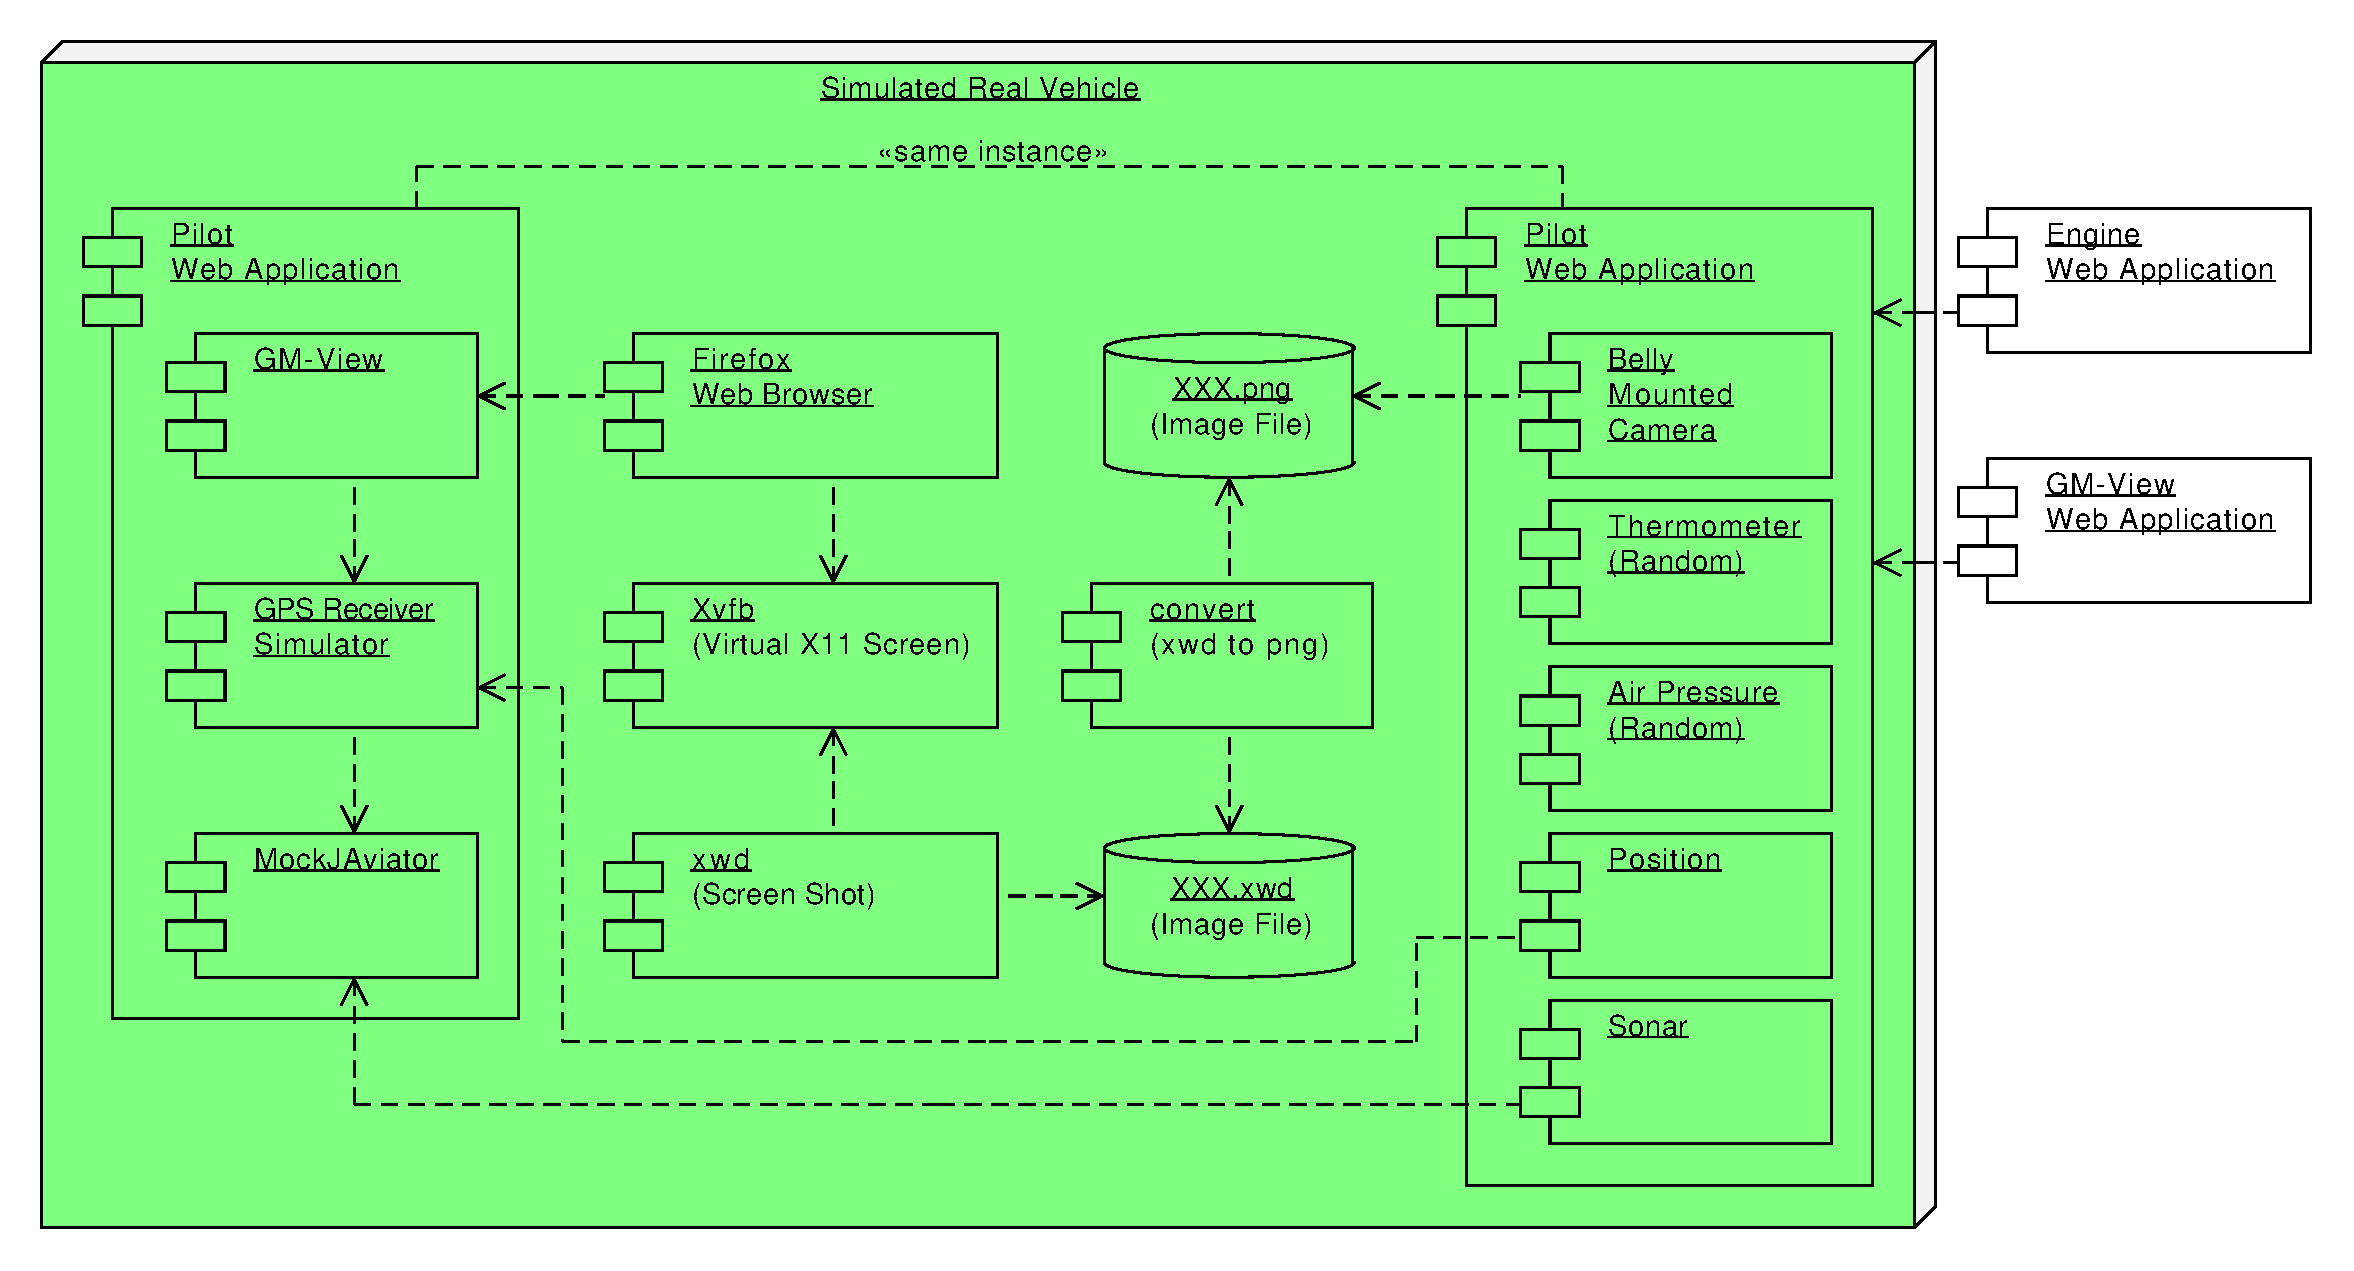
\includegraphics[width=11cm]{SensorSimulation-2.pdf}}
	\end{center}
	\caption{Sensor Simulation.\label{fig:SensorSimulation}}
\end{figure}


\section{Section}

\subsection{Subtitle}

Plain text.

\subsection{Another subtitle}

More plain text.


\section{Mapping}
The mapper is responsible for automatically mapping virtual vehicles to real vehicles. To accomplish this, the mechanism invokes 
the migration of virtual vehicles based on a mapping decision made by a mapper algorithm. The mapper is a a servlet and additionally 
to the mapper itself with its mapping algorithms, a registration service is present. The servlet can be suspended and stores all
registration information persistent in a file, otherwise registered engines would be lost. This is important because only registered 
engines are considered during the mapping process.

\subsection{Registration Service}
An engine registers itself with the registration service upon start up using its ID. If the registration was successful, the service
fetches some useful information and stores these together with the engine id. The fetched information are sensors and 
way points (flight plan), in our case, these are static informations. If a registration attempt was not successful, the engine 
keeps trying to register until it succeeds or it is terminated.

\subsection{Mapper}
The mapper itself is cyclic. It has a working and a sleeping cycle. \\
The working cycle consists of three steps:
\begin{tabbing}
1. fetch status \= of all virtual vehicles from all registered engines \\
\>	the status message includes: \= \\ 
\> \>					the next action point \\ 
\> \>					and its actions \\[0.25cm]
2. fetch status \= of all real vehicles (on which an engine is running) \\
\>	the message includes:  \\
\> \>				the current position \\
\> \> 				the next position \\
\> \>				and the velocity \\[0.25cm]
3. execute the mapping algorithm \\
\end{tabbing}
At the time of writing, there are two algorithms available that can be set in the configuration file:
\subsubsection{Random Mapping Algorithm}
Does not use any information. Randomly selects two different engines. If one of these has a virtual vehicle, then this vehicle 
will be migrated to the other engine.

\subsubsection{Simple Mapping Algorithm}

	\begin{tabbing}
	\textbf{for} \= \textbf{all} virtual vehicles \textbf{do} \\[.25cm]
	\> \textbf{if}  \= virtual vehicle program is complete \\
	\> \>	\textbf{then} invoke migration to central engine \\[.25cm]
	\>	\textbf{else} \= find fastest real vehicle with at least one needed sensor \\
	\> \>	\textbf{and} distance CurrentToNext to ActionPoint \begin{math}< \end{math} tolerance \\[.25cm]
	\>	\textbf{if} found vehicle \textbf{then} invoke migration to it \\
	\end{tabbing}

Fastest vehicle means: the vehicle with the shortest flight time from its current position to the action point (thus: higher precision \begin{math} \rightarrow \end{math} faster)
of the virtual vehicle. 

conclusion:
A virtual vehicle stays on a real vehicle or the central engine as long as there is no suitable real vehicle, but such a vehicle can't 
be hidden by a non suitable vehicle.
